\section{Dataset Construction Confounds in McDiv}\label{app:confound}

When validating against the McDiv\_nuggets benchmark \citep{tevet2020evaluating}, we observed that the mean $\bar{a}_1$ curve (per-byte) for the ``low diversity'' group starts \emph{above} the ``high diversity'' group in the story\_gen task (Figure~\ref{fig:confound-a1-dist}).
Since $a_1$ measures the surprise of the first response conditioned only on the prompt (before any other responses appear in context), this gap cannot reflect diversity.
It is a confound in the dataset construction.

\subsection{Mechanism}

The McDiv\_nuggets protocol (Tevet and Berant \S6.4) pairs a low-diversity set with each high-diversity set as follows.
Workers first write five \emph{different} continuations (the high-diversity set).
The same worker is then asked to \emph{self-select one} of their own five responses and paraphrase it five times, preserving content while varying form (the low-diversity set).
Tevet and Berant do not characterize the distribution of which responses workers self-select.

Empirically (see Table~\ref{tab:confound-stats} and Figure~\ref{fig:confound-a1-dist}, and the illustrative examples from the McDiv\_nuggets story\_gen dataset in Section~\ref{sec:mcdiv-examples} below), we observe that the self-selected endings for the low-diversity sets tend to be more specific or dramatic (e.g., ``He scored winner'' or ``they quit'') than the typical high-diversity continuations (e.g., ``Joel fired the cook when things went too far downhill'').
This means that individual low-diversity responses are intrinsically more surprising to the base model, not because of diversity, but because of the specificity of the endings workers self-selected for paraphrasing.

\subsection{Evidence}

Table~\ref{tab:confound-stats} summarizes the gap.
The per-byte $a_1$ difference is substantial (a content effect) while the total-bits difference is small because high-diversity responses are on average several bytes longer.

\begin{table*}[ht]
\centering
\caption{Unconditional surprise ($a_1$) by diversity label, McDiv\_nuggets story\_gen.}\label{tab:confound-stats}
% Generated by scripts/dataset_confound_analysis.py
% Source: results/tevet/qwen25_completion_v3/McDiv_nuggets/*_with_hds_story_gen.csv
\begin{tabular}{lccc}
\toprule
 & High diversity & Low diversity & Gap \\
\midrule
$a_1$ (bits/byte) & 0.977 & 1.154 & +0.177 \\
$a_1$ (total bits) & 49.1 & 50.5 & +1.4 \\
Mean response bytes & 52.7 & 46.5 & $-6.3$ \\
$n$ & 103 & 97 & \\
\bottomrule
\end{tabular}

\end{table*}

The gap persists after binning by response length (Table~\ref{tab:confound-length}), confirming it is primarily a content effect rather than a length artifact: the high-minus-low per-byte gap remains positive across the bulk of the length range.

\begin{table*}[ht]
\centering
\caption{Unconditional per-byte surprise by response length bin, story\_gen.}\label{tab:confound-length}
% Generated by scripts/dataset_confound_analysis.py
% Source: results/tevet/qwen25_completion_v3/McDiv_nuggets/*_with_hds_story_gen.csv
\begin{tabular}{lccl}
\toprule
Byte range & High div.\ mean & Low div.\ mean & Gap \\
\midrule
$[20, 40)$ & 1.172 & 1.340 & +0.167 \\
$[40, 60)$ & 0.878 & 1.019 & +0.141 \\
$[60, 80)$ & 0.853 & 1.029 & +0.176 \\
$[80, 120)$ & 0.905 & 0.908 & +0.003 \\
\bottomrule
\end{tabular}

\end{table*}

\subsection{Illustrative Examples}\label{sec:mcdiv-examples}

Figures~\ref{fig:confound-high} and~\ref{fig:confound-low} show per-token surprise (in bits) for the first response of a high-diversity and low-diversity sample, respectively.
Samples are drawn by ranking each label group by per-byte $a_1$ (ascending for high-diversity, descending for low-diversity) and taking the sample at the $\lfloor N/4 \rfloor$ position, chosen to be representative of the expected confound direction rather than an extreme outlier; the specific pinned IDs (\texttt{sa\_00698}, \texttt{sa-b\_00279}) are fixed in \texttt{scripts/dataset\_confound\_analysis.py} for reproducibility.
Red bars are measured response tokens; grey bars are masked context tokens.

\paragraph{High diversity} (Figure~\ref{fig:confound-high}).
Context: \emph{``Joel owned a restaurant.
He hired a cook that didn't care about his work.
The cook didn't clean after himself.
The kitchen was a mess.''} Response: \emph{``Joel fired the cook when things went too far downhill.''} This is a natural, predictable continuation ($a_1 = \confoundHighRoAone$ bits/byte).

\paragraph{Low diversity} (Figure~\ref{fig:confound-low}).
Context: \emph{``Harry and his basketball team was losing the game.
The coach called for a timeout.
Harry boosted morale by talking to his team.
The team caught up and the game was tied.''} Response: \emph{``He scored winner.''} This is a specific, somewhat ungrammatical ending ($a_1 = \confoundLowRoAone$ bits/byte).
All five responses in this set are paraphrases of the same idea (``Harry scored the winning point'').

\begin{figure*}[h]
\centering
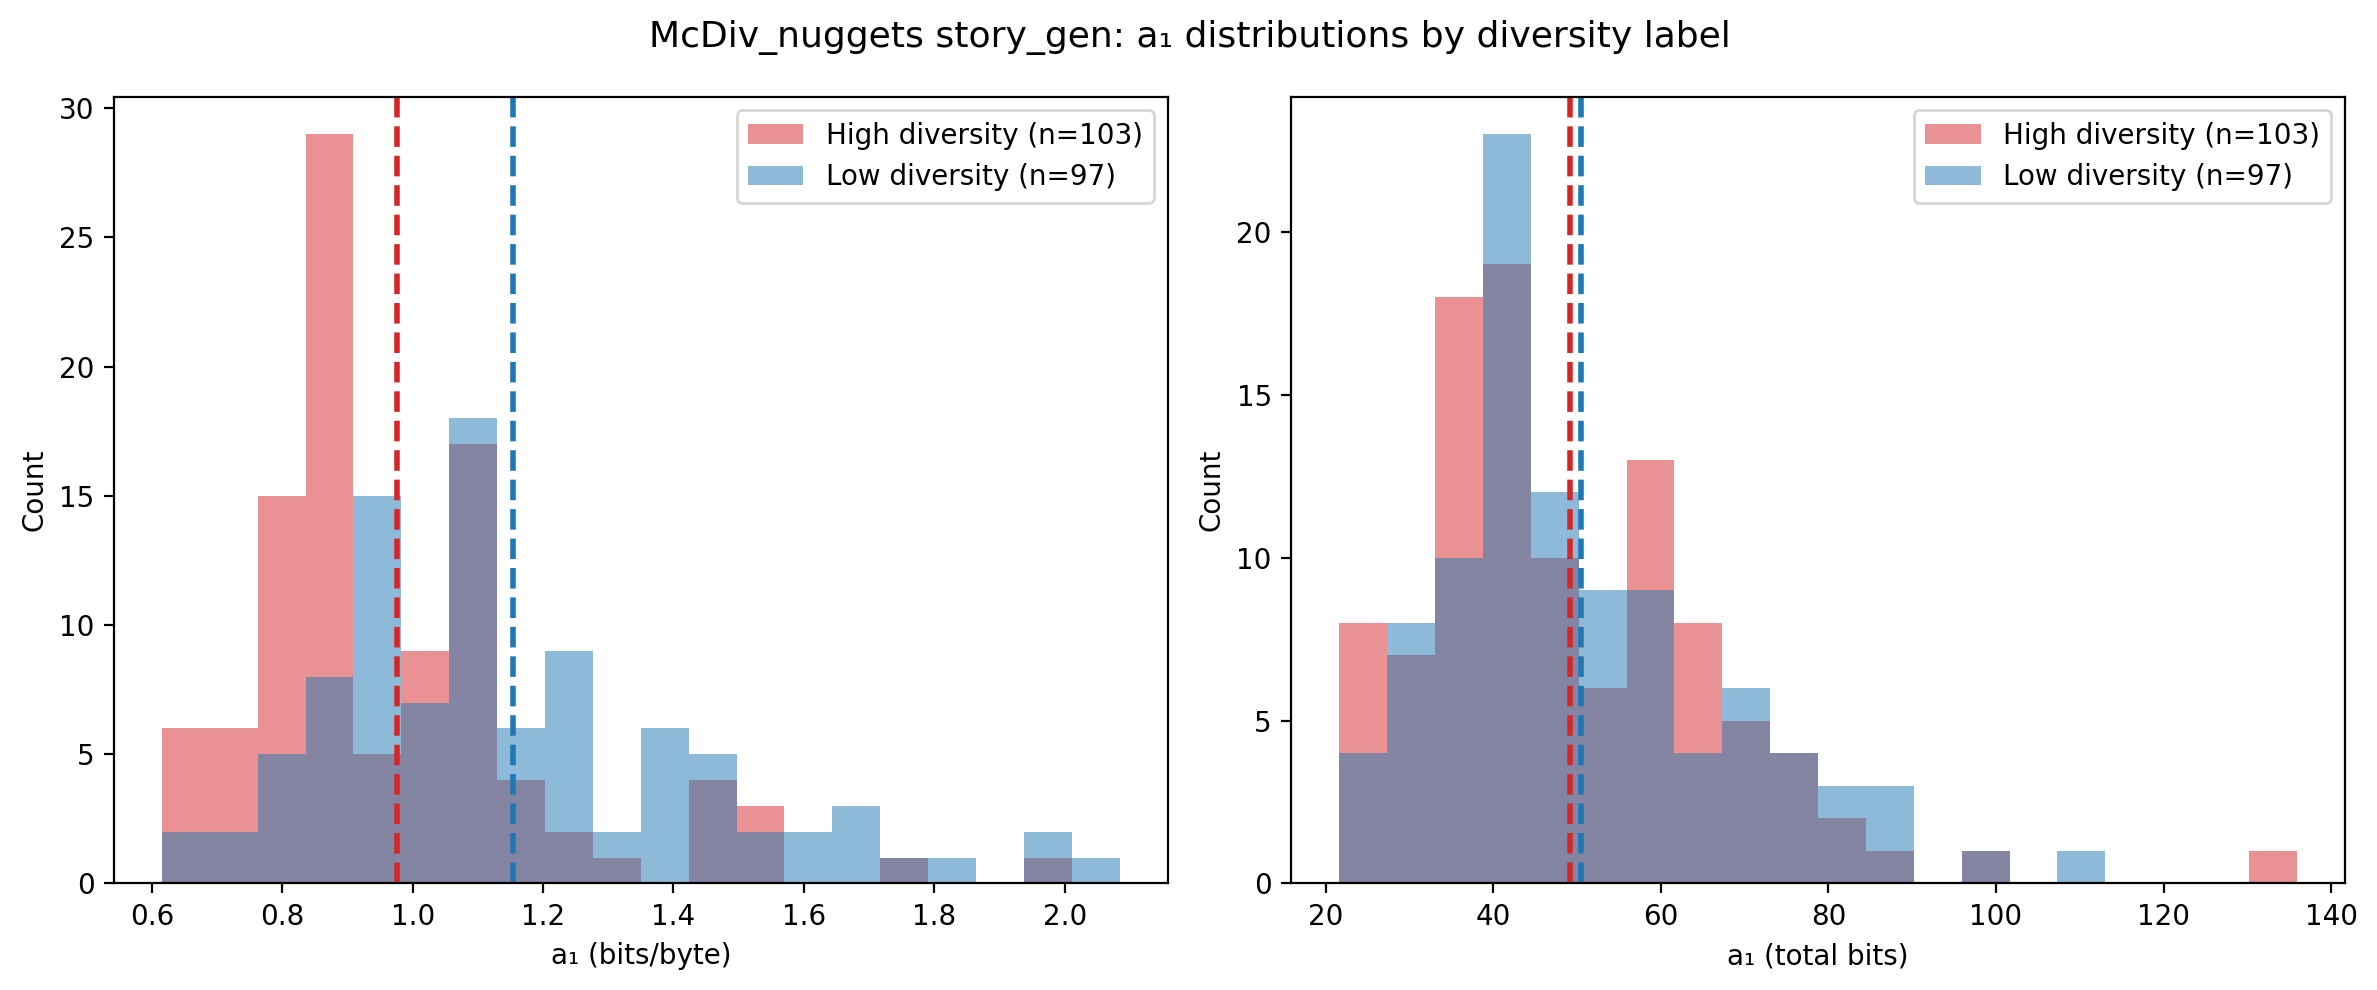
\includegraphics[width=\textwidth]{../figures/dataset_confound/a1_distributions.png}
\caption{Distribution of $a_1$ (unconditional surprise of the first response) for high- vs.\ low-diversity story\_gen samples.
Left: per-byte.
Right: total bits.
The per-byte gap (see Table~\ref{tab:confound-stats}) is a dataset construction artifact.}\label{fig:confound-a1-dist}
\end{figure*}

\begin{figure*}[h]
\centering
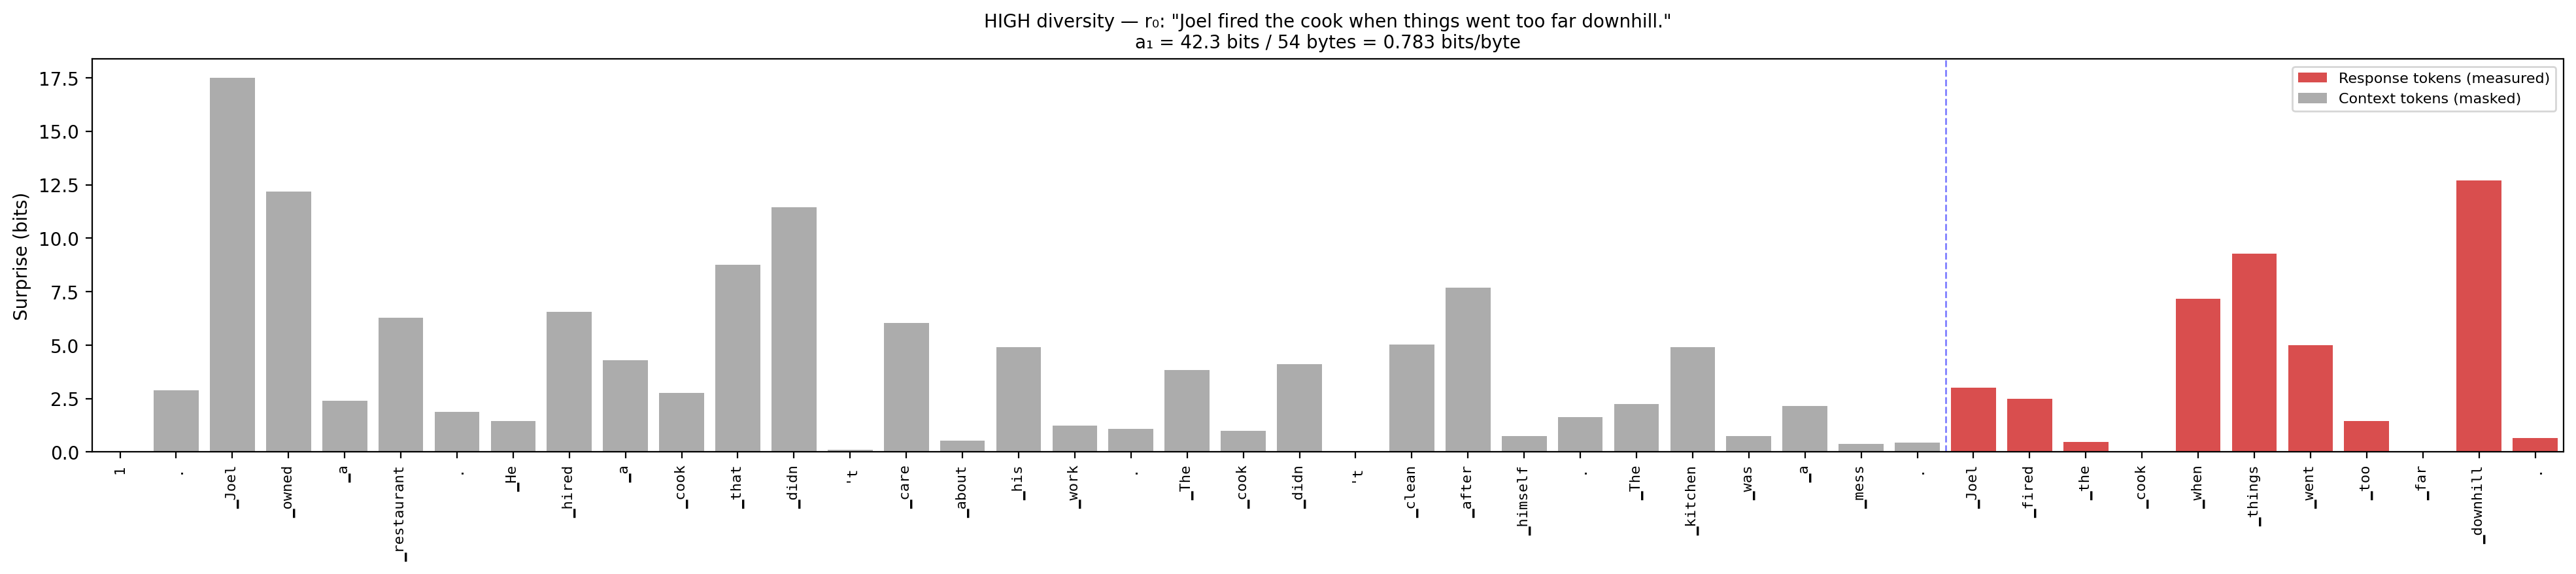
\includegraphics[width=\textwidth]{../figures/dataset_confound/per_token_high_0_test.sa-sb.sa_00698.png}
\caption{Per-token surprise for a high-diversity sample's first response.
The continuation (``Joel fired the cook...'') is predictable, yielding low per-token surprise across response tokens.}\label{fig:confound-high}
\end{figure*}

\begin{figure*}[h]
\centering
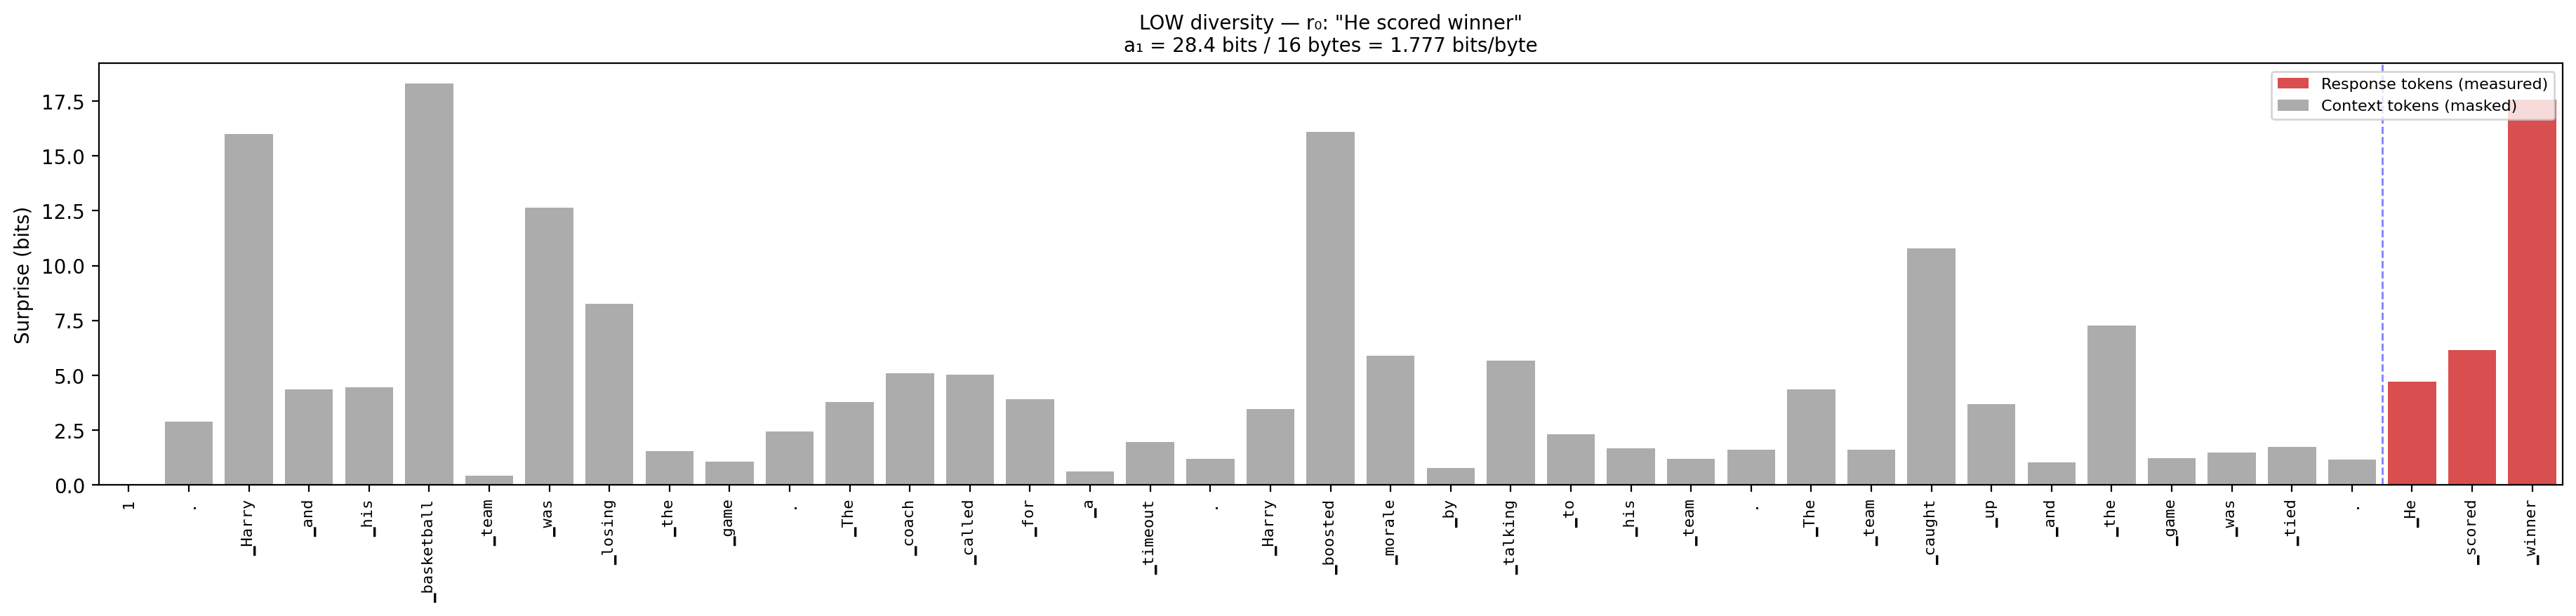
\includegraphics[width=\textwidth]{../figures/dataset_confound/per_token_low_0_test.sa-sb.sa-b_00279.png}
\caption{Per-token surprise for a low-diversity sample's first response.
The specific ending (``He scored winner'') is inherently more surprising to the base model, despite being labeled ``low diversity.''}\label{fig:confound-low}
\end{figure*}

\subsection{Label Contamination}

In addition to the construction confound, we found that the McDiv\_nuggets CSVs contain duplicate sample IDs with \emph{conflicting labels}: the same response set appears once labeled as high diversity and once as low diversity.
Table~\ref{tab:contamination} shows the extent of this contamination across the three generation tasks.

\begin{table*}[ht]
\centering
\caption{Number of sample IDs appearing with both high- and low-diversity labels in the McDiv\_nuggets (with HDS) CSVs.}\label{tab:contamination}
% Generated by scripts/dataset_confound_analysis.py
% Source: results/tevet/qwen25_completion_v3/McDiv_nuggets/*_with_hds_*.csv
\begin{tabular}{lcc}
\toprule
Task & Conflicting IDs & Total rows \\
\midrule
prompt\_gen & 9 & 200 \\
resp\_gen & 11 & 200 \\
story\_gen & 7 & 200 \\
\bottomrule
\end{tabular}

\end{table*}

These duplicates introduce noise into any correlation analysis: the same $\bar{a}_k$ curve is counted as evidence for \emph{both} labels, diluting the signal.
We did not remove these duplicates from our analysis, so the correlations reported here are conservative.

\subsection{Implications}

This confound does not invalidate McDiv\_nuggets for evaluating diversity metrics, but it does introduce a systematic bias: any metric based on per-response surprise will tend to assign higher values to the low-diversity group, counteracting the expected positive correlation between the metric and the diversity label.
Metrics that compare \emph{across} responses within a set (like excess entropy $E$) are less affected because the confound is approximately constant across positions $k$: it shifts the entire $\bar{a}_k$ curve vertically without changing its shape.
Per-byte normalization amplifies the confound because shorter low-diversity responses get higher bits-per-byte values.

